\chapter{Introduction}
\label{cha:introduction}

With the proliferation of new technologies, the amount of data will drastically increase and certainly empower new innovations. In fact, the worldwide interaction with data follows an exponentially growing trend, with a volume of 79 \acrfull{zb} in 2021, and an expected volume of 181 \acrshort{zb} in 2025 \cite{statistaDataWorldWide}. This giant pool of data can help companies to develop new business models, make better decisions through analytics and build smarter applications with machine learning models. For example, access to data can enhance the treatment of diseases in the healthcare sector \cite{koutsosAgoraPrivacyAwareData,wangBigDataAnalytics2018,suBDTFBlockchainBasedData2020} and increase productivity and efficiency in the agriculture sector \cite{elijahOverviewInternetThings2018}. More and more connected \acrfull{iot} devices accelerate the collection of valuable data \cite{ozyilmazIDMoBIoTData2018,lawrenzBlockchainTechnologyApproach2019}, however, without open and censorship-free access it cannot be used.

On the flip side, tech giants such as Meta, formerly Facebook Inc., have access to a large volume of data and thus take advantage of their monopoly for their own profit \cite{serranoPeertoPeerOwnershipPreservingData2021}. They especially abuse \acrfull{pii} of each user profile to tailor targeted advertisements which accounts for 99\% \cite{GlobalMetaAdvertising} of their yearly revenue \cite{arrategalanLargeScaleAnalysisUser2019}. Considering the fact that lately 2.9 billion monthly active users \cite{FacebookMAUWorldwide} are worth around \$9.41 \cite{FacebookAverageRevenue} each, Meta's yearly revenue is tremendous with data that is actually owned by their users. Moreover, Meta outrageously gave \acrshort{pii} of more than 87 million users to Cambridge Analytica without consent \cite{isaakUserDataPrivacy2018,xiaoPrivacyGuardEnforcingPrivate2020}. Given the economical value and the lack of open and censorship-free access to data for \emph{everyone}, this inevitably leads to the question: "What if every individual can decide on their own, what data they share and how they monetize it to earn profit?". This consequently promotes the need for a trustable and neutral online data trading platform for data buyers and sellers -- a so-called data marketplace \cite{dagevilleSnowflakeElasticData2016,krishnamachariI3IoTMarketplace2018}.

%Those who sell data may be individuals who want to take advantage of the data generated by their mobile phones, smartwatches, biomedical sensors and other IoT gadgets; but most of the times, these are companies that want to monetize the content of their databases and use the proceeds to continue growing.

% A conventional data marketplace is a two-party trading platform, where data owners, referred to as sellers \emph{S}, monetize valuable data to get compensated for data access by interested parties, referred to as buyers \emph{B} \cite{banerjeeBlockchainEnabledData2019}. Such conventional two-party data marketplaces have one thing in common -- it is not possible to guarantee fair exchange, i.e. receiving legitimate data as \emph{B} while receiving the agreed-upon payment as \emph{S}, without a Trusted Third Party (TTP) \cite{banerjeeBlockchainEnabledData2019}. Hence, the two-party model is typically extended by a centralized trading platform, where \emph{S} uploads and advertises his or her data, and the platform sells it on behalf of \emph{S} \cite{banerjeeBlockchainEnabledData2019,daiSDTESecureBlockchainBased2020,suBDTFBlockchainBasedData2020}.

% A conventional data marketplace is a two-party trading platform, where data owners, referred as sellers \emph{S}, monetize their valuable data to get compensated for data access by interested parties, referred as buyers \emph{B} \cite{banerjeeBlockchainEnabledData2019}. Such data marketplaces come in different variations. For example, there are paid subscription models for an interface to dynamic real-time data in contrast to a one-time-purchase model for access to a static resource. In addition, data marketplaces can be classified as Business-to-Business (B2B) or Business-to-Consumer (B2C) platforms. %Examples and citation or only citation?).
% However, all conventional two-party data marketplaces have one thing in common -- it is not possible to guarantee fair exchange, i.e. receiving legitimate data as \emph{B} while receiving the agreed-upon payment as \emph{S}, without a Trusted Third Party (TTP) \cite{banerjeeBlockchainEnabledData2019}. Hence, the two-party model is typically extended by a centralized trading platform, where \emph{S} uploads and advertises his or her data, and the platform sells the data on behalf of \emph{S} \cite{banerjeeBlockchainEnabledData2019,daiSDTESecureBlockchainBased2020,suBDTFBlockchainBasedData2020}.


% spof nennen und data breach
% while trust issues are mitigated by fairswap, review systems etc. some problems remain -> also problematic when data leaves boundaries, regulation, privacy
% ownership, trust, privacy, regulation problems nennen -> blockchain kann nur trust und transparency etc. lösen!
A conventional data marketplace is typically a centralized platform with a \acrfull{ttp} that facilitates the data exchange between a buyer and seller \cite{daiSDTESecureBlockchainBased2020}, just like eBay\footnote{https://www.ebay.com/} or Amazon\footnote{https://www.amazon.com/} does with physical goods. However, a malicious and biased platform might take advantage of its monopoly to advertise products and distort rankings for its own profit \cite{ramachandranDecentralizedDataMarketplace2018}. Even worse, once the seller transmits raw datasets to the platform, it might resell them without consent \cite{suBDTFBlockchainBasedData2020,serranoPeertoPeerOwnershipPreservingData2021,daiSDTESecureBlockchainBased2020,banerjeeBlockchainEnabledData2019}. Hence, a centralized platform is a \acrfull{spof} that can lead to significant data breaches. A decentralized infrastructure might help to mitigate issues with regard to trust \cite{ramachandranDecentralizedDataMarketplace2018}. Blockchain technology, first introduced in 2008 by Satoshi Nakamoto \cite{nakamotoBitcoinPeertoPeerElectronic}, inherently provides a promising approach by providing "immutability and transparency of cryptographically-secured and peer-recorded transactions, which have been agreed upon by network consensus" \cite{eberhardtBlockchainInsightsOffChaining2017}.

%One who buys data normally ends up with a copy of the raw data, which he can resell to other parties as many times as he wants, without giving any contribution to the rightful data owner, sometimes even despising non-disclosure agreements. peer to peer

%A dishonest seller \emph{S} may be tempted to refuse access or return manipulated data after receiving the payment \cite{suBDTFBlockchainBasedData2020,lawrenzBlockchainTechnologyApproach2019}. On the opposite, a dishonest buyer \emph{B} may be tempted to never pay the price after receiving the purchased dataset \cite{lawrenzBlockchainTechnologyApproach2019}. 
%This is a form of piracy and, depending on the type of data, can violate privacy. All in all, a centralized platform is a \acrfull{spof} \cite{daiSDTESecureBlockchainBased2020} that is not able to satisfy \emph{Fairness}, \emph{Transparency}, \emph{Security}, \emph{Privacy}, and non-discrimination, among others \cite{banerjeeBlockchainEnabledData2019}. 

%Any digital data marketplace, whether centralized or decentralized, needs some specific key components and features. This includes: (i.) \emph{Fairness}; (ii.) \emph{Transparency}, \emph{Privacy} and \emph{Security}; (iii.) \emph{Regulation}; as well as (iv.) \emph{Efficiency}, according to Banerjee and Ruj \cite{banerjeeBlockchainEnabledData2019}. Ramachandran et al. \cite{ramachandranDecentralizedDataMarketplace2018} complements this by functional requirements such as: (v.) \emph{Posting and Discovery}; (vi.) \emph{Data Transfer and Payments}; (vii.) \emph{Metadata Organization}; (viii.) \emph{Data Quality - Buyer and Seller Ratings}; (ix.) \emph{Data Quality - Curation and Recommendations}; and (x.) \emph{Identity - and Access Control Management (IAM)}. These requirements are surrounded by the buyer and seller, as depicted in Figure \ref{fig:components}.

%\begin{figure}[!htb]
%    \centering
%    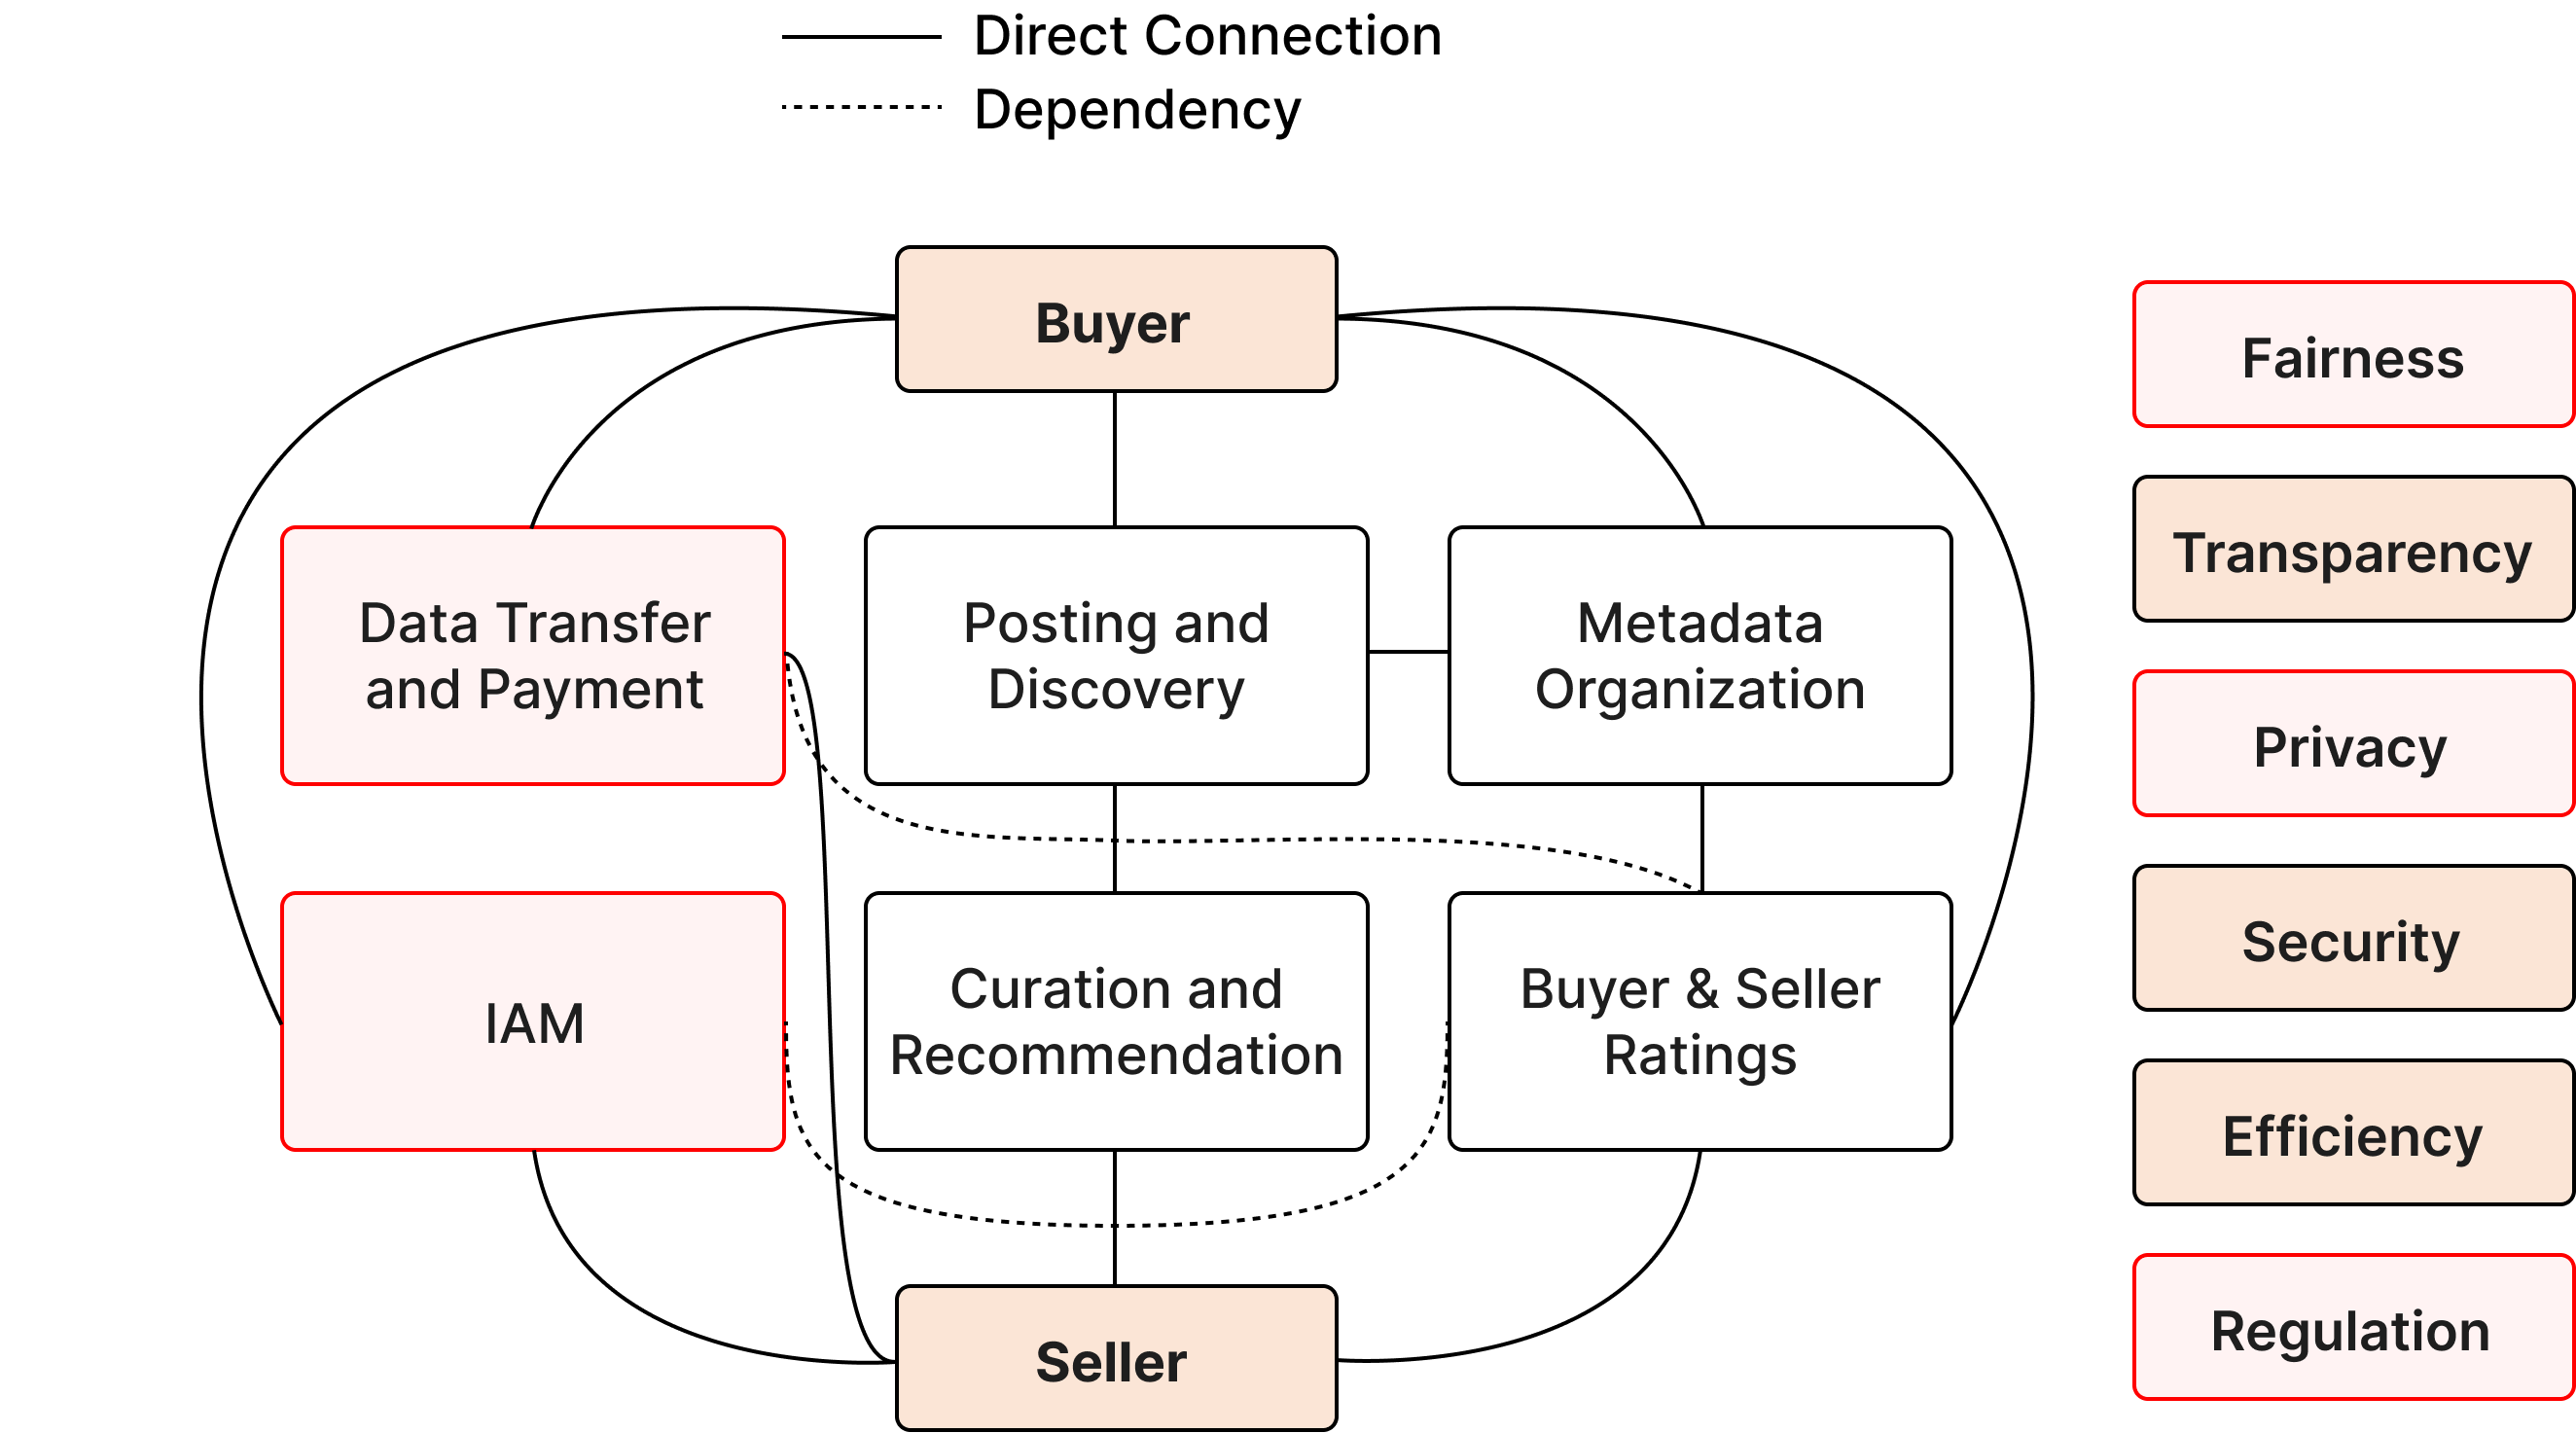
\includegraphics[width=13cm]{images/components.png}
%    \caption[Key components and features of a digital data trading platform]{Key components and features of a digital data trading platform. All components in red show the aspired enhancements by the contributions of this thesis.}
%    \label{fig:components}
%\end{figure}

%"Blockchain-based application architectures benefit from a set of unique properties including immutability and transparency of cryptographically-secured and peer-recorded transactions, which have been agreed upon by network consensus" \cite{eberhardtBlockchainInsightsOffChaining2017}. According to that, it is trivial to implement sufficient \emph{Transparency} and \emph{Security} in blockchain-based data marketplaces. Furthermore, it turns out the non-trivial \emph{Fairness} problem in a two-party trading relationship seems to be solved by Blockchain technology in one atomic swap \cite{dziembowskiFairSwapHowFairly2018,liZKCPlusOptimizedFairexchange2021}. However, \emph{Privacy}, \emph{Regulation} and \emph{Efficiency} remains a bigger problem for blockchain-based data marketplaces due to limitations of public permission-less Blockchains such as Bitcoin \cite{nakamotoBitcoinPeertoPeerElectronic} and Ethereum \cite{buterinNEXTGENERATIONSMART}.

%Public permission-less Blockchains inherently validate and process transaction data at every node, in order to guarantee network consensus. By virtue of its design, all data is available at each node which makes this system purposely public in favor of transparency properties. However, data sharing often incorporates \acrfull{pii} and confidential data. Consequently, storing and computing private data on these ledgers is conflicting with Privacy requirements, enforced by regulations such as the \acrfull{gdpr} \cite{european_commission_regulation_2016}. In any case, it is not advisable to store large amounts of data in Blockchains due to block-size limitations, Blockchain bloating and extremely high associated storage costs.

%Off-chain storage solutions are suggested to overcome this limitation. In particular the Content-Addressable Storage Pattern \cite{eberhardtBlockchainInsightsOffChaining2017} seems to be a reasonable solution to store large amounts of data while keeping key properties of Blockchains such as immutability. Decentralized peer-to-peer networks such as IPFS \cite{benetIPFSContentAddressed2014}, Filecoin \cite{filecoin} and SWARM \cite{swarm} provide a promising approach to that. However, these networks suffer from the same Privacy issues as Blockchains due to open access and data replication across the network.

%Another problem seems to be the enforcement of access and usage regulations in a distrusted setting without a \acrfull{ttp}. A seller loses full control over his data when the buyer receives it. Hence, he or she is not able to enforce geographical usage restrictions or purpose limitations for example. This especially violates the principle of purpose limitation codified in Art. 5 of the \acrshort{gdpr} \cite[Art. 5 (1 b)]{european_commission_regulation_2016}. Given a malicious buyer, he or she might even resell the purchased dataset without the seller's knowledge.

No matter if centralized or decentralized infrastructure, it is observable that most problems occur when data leaves the boundaries of the seller, i.e. raw datasets are moved to an intermediate storage platform and/or the buyer, to be processed. In a naive approach, sellers would encrypt raw datasets in the first place, however, \emph{Ownership}, \emph{Privacy}, and \emph{Regulation} still remain a problem, once they are decrypted by the buyer or the buyer loses decryption keys. Accordingly, we suggest flipping the strategy, i.e. raw datasets never leave the boundaries of the seller, such that only a computation over the dataset is moved to the buyer, thereby protecting \acrshort{pii} and confidential data. This paradigm is referred to as \emph{\acrfull{c2d}}. However, a problem with this paradigm is that, given a malicious seller, the buyer cannot verify if the result has been computed correctly. \acrfull{voc} has been suggested to address this problem \cite{eberhardtBlockchainInsightsOffChaining2017,eberhardtOffchainingModelsApproaches2018}.

% im gegensatz zu physical goods haben daten nur wert wenn sie korrekt sind!!!!!!!!!!!!!!!

%Verifiable Off-chain Computation (VOC) has been suggested to address this problem \cite{eberhardtOffchainingModelsApproaches2018,eberhardtBlockchainInsightsOffChaining2017}.

%Thereby, we make two individual contributions ...:

This thesis presents a practical real-world implementation of a blockchain-based data marketplace for verifiable computations on private datasets. Accordingly, buyers can discover interesting datasets on the marketplace and purchase arbitrary computations such as an average of some hidden data records. Sellers instead are responsible for executing those computations within their boundaries and for submitting the result along with a verifiable proof of computational correctness. Thereby, the proposed solution enhances \emph{Ownership}, \emph{Privacy}, and \emph{Regulation} in blockchain-based data trading platforms with a focus on static infrequently changing datasets as opposed to real-time streaming data and training of machine-learning models. Specifically, this thesis leverages \acrshort{voc}, in particular a \acrfull{zkp} protocol, implemented with the ZoKrates\footnote{https://github.com/Zokrates/ZoKrates} toolbox, to cryptographically prove computational correctness on the Ethereum blockchain. Additionally, blockchain technology is used to (i.) process payments; (ii.) create a transparent, non-repudiable, and tamper-proof log of events; and (iii.) enforce data usage policies. Thereby, the contribution of this thesis is threefold:

\begin{enumerate}
    \item What components are mandatory for a blockchain-based data marketplace and how can the \acrlong{c2d} paradigm be applied?
    \item How can the \acrlong{c2d} paradigm be made verifiable without sacrificing ownership, privacy and regulation?
    %\item How practical is the proposed solution?
    \item An evaluation on the practicality of the proposed solution is provided.
\end{enumerate}

The remainder of this thesis is organized as follows: Chapter \ref{cha:background} provides fundamental background knowledge to understand the remainder of this thesis. Chapter \ref{cha:relatedwork} gives a brief overview of the current research, with regard to privacy-aware blockchain-based data marketplaces. Chapter \ref{cha:requirements} summarizes the functional and non-functional requirements for the desired software artifact outcome. The concept \& design of the software artifact is outlined in Chapter \ref{cha:cod} and its implementation is explained in Chapter \ref{cha:implementation}. Lastly, Chapter \ref{cha:evaluation} evaluates and discusses the implementation based on the defined requirements, followed by a conclusion in Chapter \ref{cha:conclusion}, to summarize the results and ideas for future work.


% https://ieeexplore.ieee.org/stamp/stamp.jsp?arnumber=9739681
%Compute-to-data has already been discussed as an access
%method in section III-A, but it is also a solution that addresses
%problems of transaction enforcement, as well as maintaining
%data governance. With compute-to-data, rather than handing
%over the data to the data consumer for consumption in their
%environment, the consumer sends code to manipulate the data
%and receives results of computation that generally do not
%expose the underlying data. In its simplest form, the data
%provider sends the code directly to the data provider, who
%either provides an environment for execution of the code
%or runs the code manually themselves [19], [52]. However,
%since code can also be considered a data product, the data
%consumer might not be willing to share their code for the
%same reasons the data provider is not. In such a case, a trusted
%third party can be charged with providing an isolated environment where the code can be executed on the data [31], [34].
%A special case of compute-to-data is the use of multi-party
%computation whereby code is run on multiple data products
%in multiple physical locations, and an aggregate result is
%obtained without revealing information from the individual
%data products [147].

% dataset: https://archive.ics.uci.edu/ml/datasets/daily+and+sports+activities#
% https://archive.ics.uci.edu/ml/datasets.php